Thinking...
The user asks: "以下のの日本語文を英訳してください。ただしTeXのコードが挿入されているのでその部分はそのまま出力してください： [TeX figure environment]". So we need to translate the Japanese text (which includes some Japanese in caption: "各グループの雑誌の構成に関するKLD") into English, while keeping the TeX code unchanged. So likely output the same LaTeX block but with caption translated. The rest of the text maybe just the figure environment. So we need to replace the caption text with English translation: "KLD of the composition of magazines for each group" or similar. Also maybe translate other parts like "各グループの雑誌の構成に関するKLD" => "KLD regarding the composition of magazines for each group". The rest (figure, label) remain same. The user said "以下のの日本語文を英訳してください" (translate the following Japanese sentence into English). The only Japanese part is the caption. So output the TeX code with caption in English. Provide translation maybe outside? But they said output the same code with unchanged TeX parts. So final answer should be the code block with caption translated. Let's do that.

...done thinking.

\begin{figure}[h]
\begin{center}
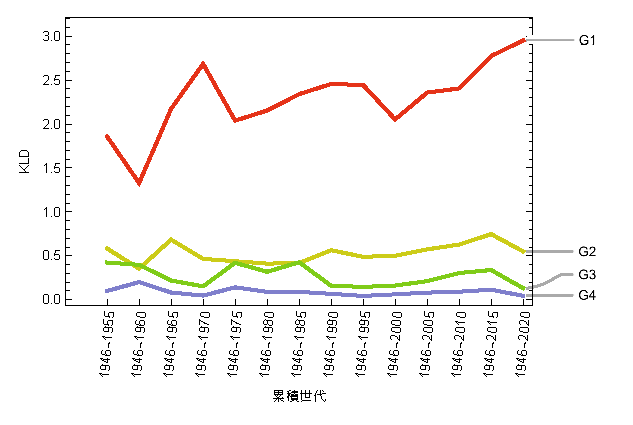
\includegraphics[width=76mm]{gr12.eps}
\caption{KLD regarding the composition of magazines for each group}
\label{fig:gr12}
\end{center}
\end{figure}

